% !TeX spellcheck = en_US 
\chapter{Forensic audit and its computer support}


\komentar{na zacatek shrnout co vsechno obsahuje tato kapitola. asi tak takhle:}


This chapter strives to define and explain the meaning of the term "forensic audit" as well as other therms related to this field. We demonstrate typical roles and outline the process.
\komentar{az bude kapitola dopsana, zkontrolovat, zda toto odpovida} 

\section{Matters of forensic audit}
\komentar{nelibi se mi, pridat do jinych casti a zrusit}
Forensic audit is a specialization within a field of accounting that examines and evaluates evidence concerning unproven statements for possible use as evidence in court. Forensic audit is usually used in case there is a suspicion in certain company there is a crime being committed. The background of the investigated case is rather diverse. A customer can be, for example, a CEO  who wants to examine the functioning of one of the sub-divisions of a controlling company. There can be a suspicion of some fraudulent activity or the need of forensic audit can be closely unspecified.

\section{What is forensic audit}
The term "forensic" can be defined in multiple ways. According to merriam-webster dictionary \komentar{citace http://www.merriam-webster.com/dictionary/forensic} the definition is "relating to the use of scientific knowledge or methods in solving crimes". The term "audit" is explained in the same dictionary as "a complete and careful examination of the financial records of a business or person". \komentar{citace http://www.merriam-webster.com/dictionary/audit}

The essence of forensic audit is to discover and investigate fraudulent intentions and fraudulent behavior. 

A common mistake in the definition of forensic audit is to confuse it with financial audit. The aim of financial audit is to verify whether financial statements are fairly stated in accordance with accounting standards. Financial auditors search for material errors or other misstatements in the accountancy.

On the other hand the ultimate goal of forensic audit is to examine existing or gained suspicion and procure evidence concerning possible fraudulent behavior. Deceptive scenarios are discovered in the process of forensic audit and evidence together with a documentation that is usable for subsequent course of action is gathered. As a matter of principle forensic auditors are not expected to express their opinion on the guilt or innocence of suspects.


\section{When to use forensic audit}
\sediva{\blindtext}


\section{How to prepare for a forensic audit}
\komentar{v hrubych rysech jak to probiha (to co uz mam sem patri), na zaklade toho, co jsem zjistila, FA funguje takto:...\\}

On the basis of what we have found the process of forensic audit works as follows. When it is decided that certain situation will be investigated in forensic audit it is important to prevent all investigated individuals to access all related documents and electronic evidence. It is also recommended to limit their access to corporate information systems. 

Next step is to formulate properly the assignment. To define the extent and expectations on the outcome of forensic audit. To prevent a misunderstanding the assignment should be as specific and detailed as possible. It is best to choose the right audit company according to references and their experience with similar cases as the one we have specified.

When a client contacts an audit company with an assignment they usually schedule a meeting together formulate and sign and accept the assignment. The ordering party should be prepared to provide access to corresponding electronic and paper-like documentation as well as accept the fact that auditors are going to question employees and case-related person. On the other hand the audit company undertakes to refrain from sharing all the confidential information with third parties.A team of specialists that are convenient to the assignment is formed and the inspection is launched. 

The following steps of the precise method of forensic audit are not definite. The ability to adapt in new situations is one of many essential capabilities for the team of forensic auditors. The variety of investigated cases is so vast that there is no universally valid and precise course of action in the same time. Therefore on this place we present only general methodology of forensic audit. Several selected methods of forensic audit will be described later in this document. \komentar{link na spravne misto!}

\section{General methodology of forensic audit}



\sediva{\blindtext}





\begin{figure}[h]
	\begin{center} 
	\missingfigure{Obrazek demonstrujici forenzni audit.}
	%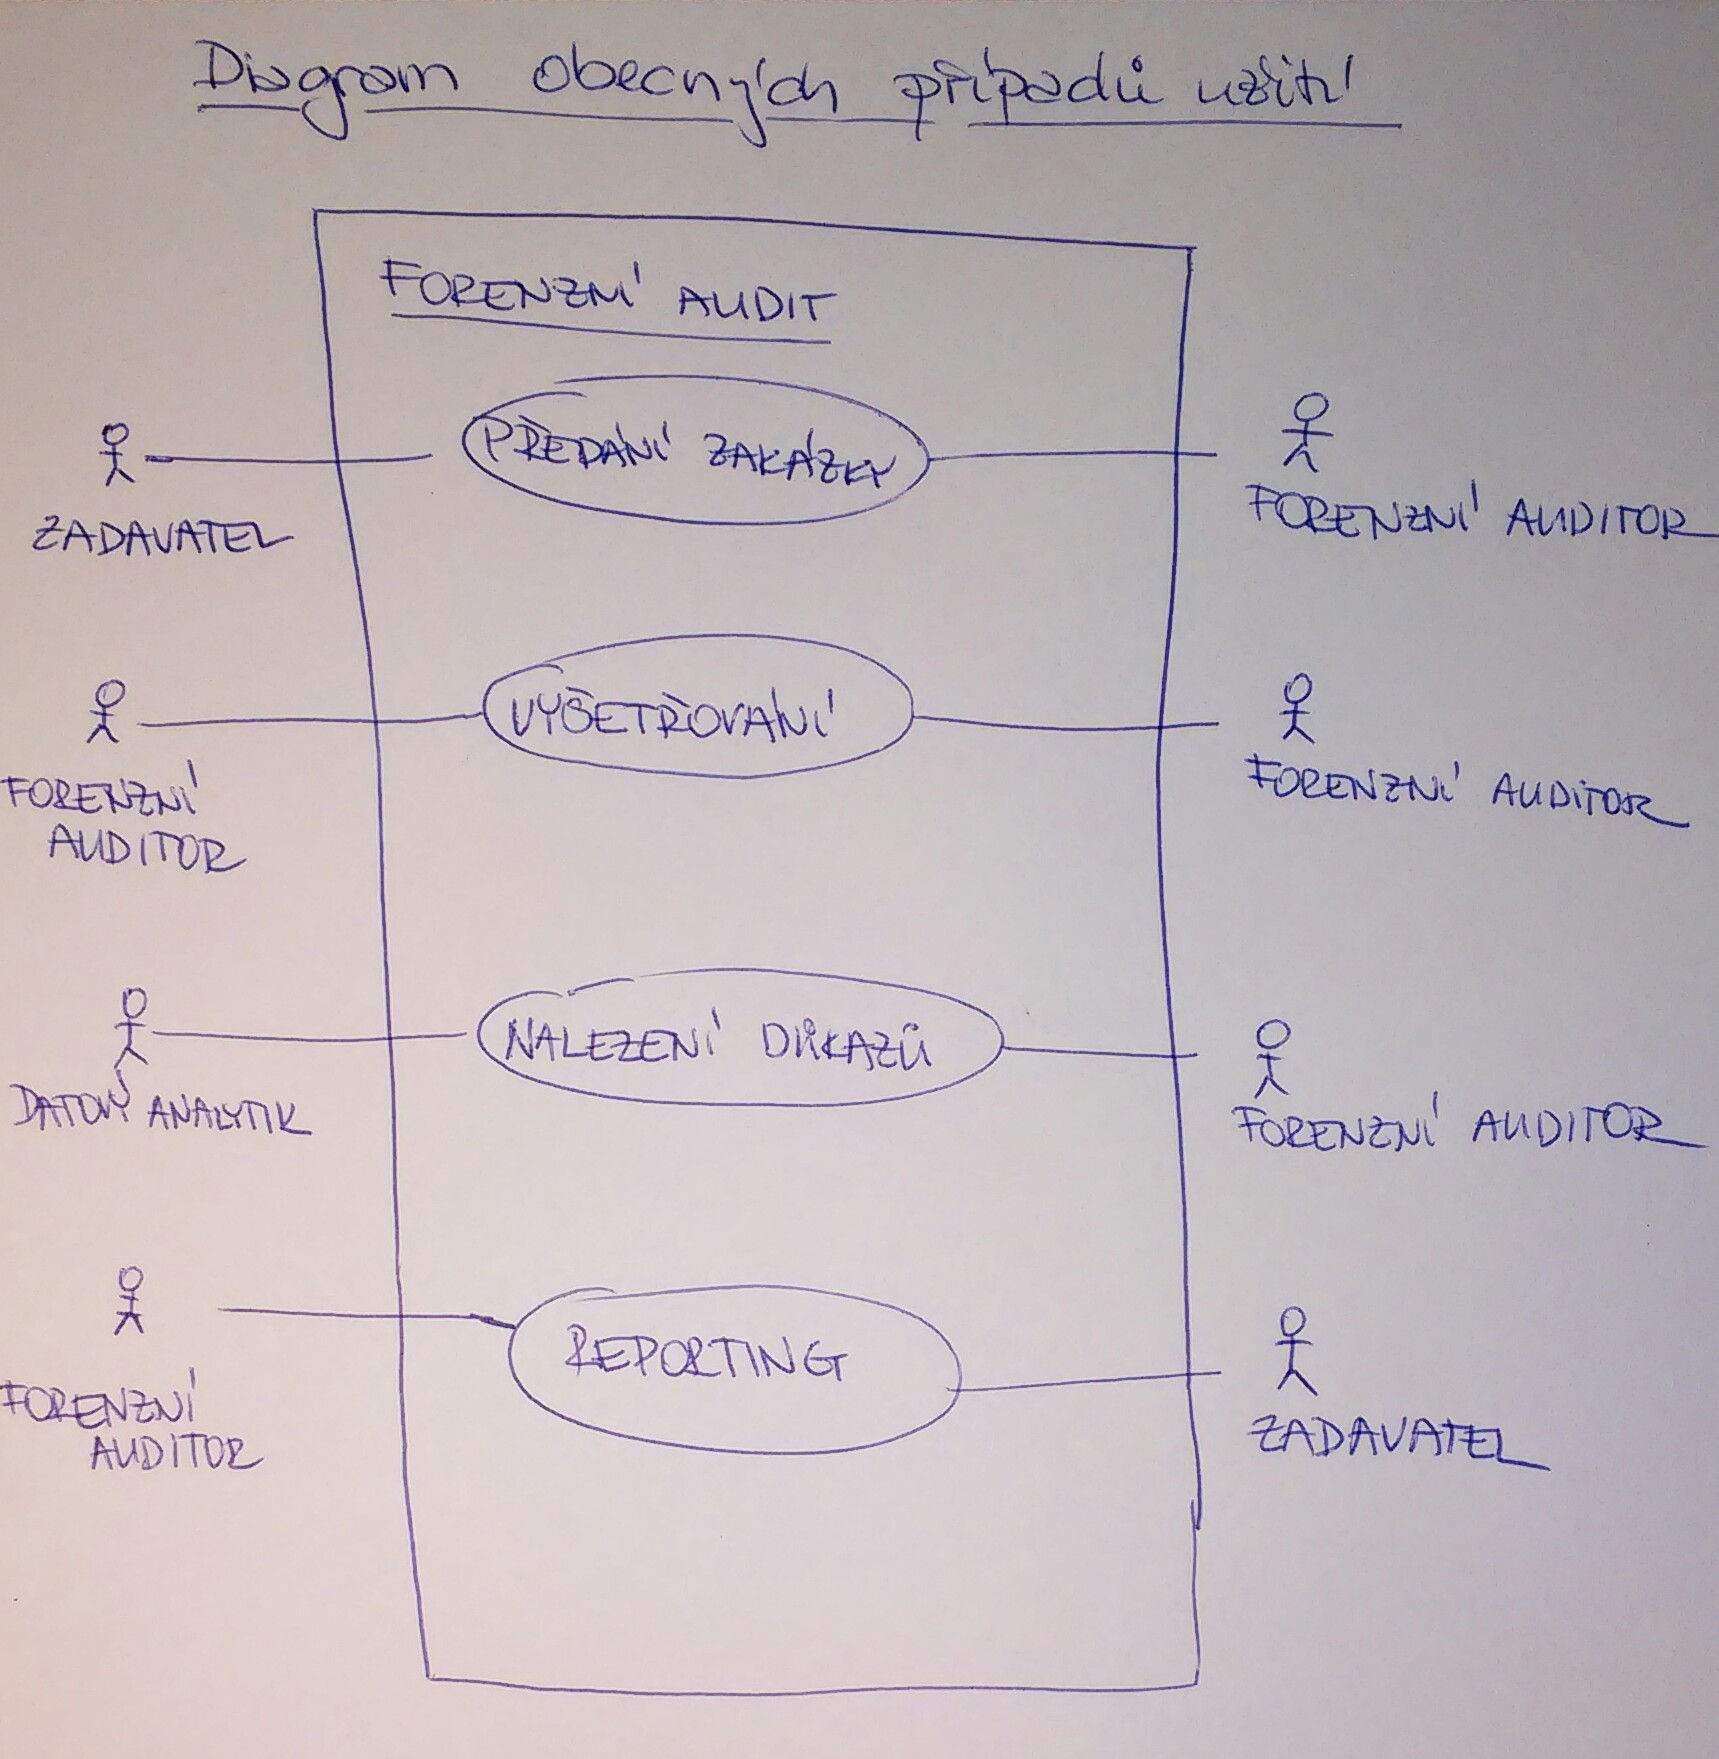
\includegraphics{img/fotky/20151007_000323.jpg}
	\end{center}
	\caption{\komentar{Obrazek demonstrujici forenzni audit.}}
\end{figure}





\section{use case diagram}
\komentar{ komentar k diagramu}


\sediva{ \blindtext}

\begin{figure}[h]
	\begin{center} 
	%\missingfigure{Velky obrazek vsech zainteresovanych stran - f.auditor, datovy analytik pro FA, zakaznik (zadavatel, materska spolecnost)}
	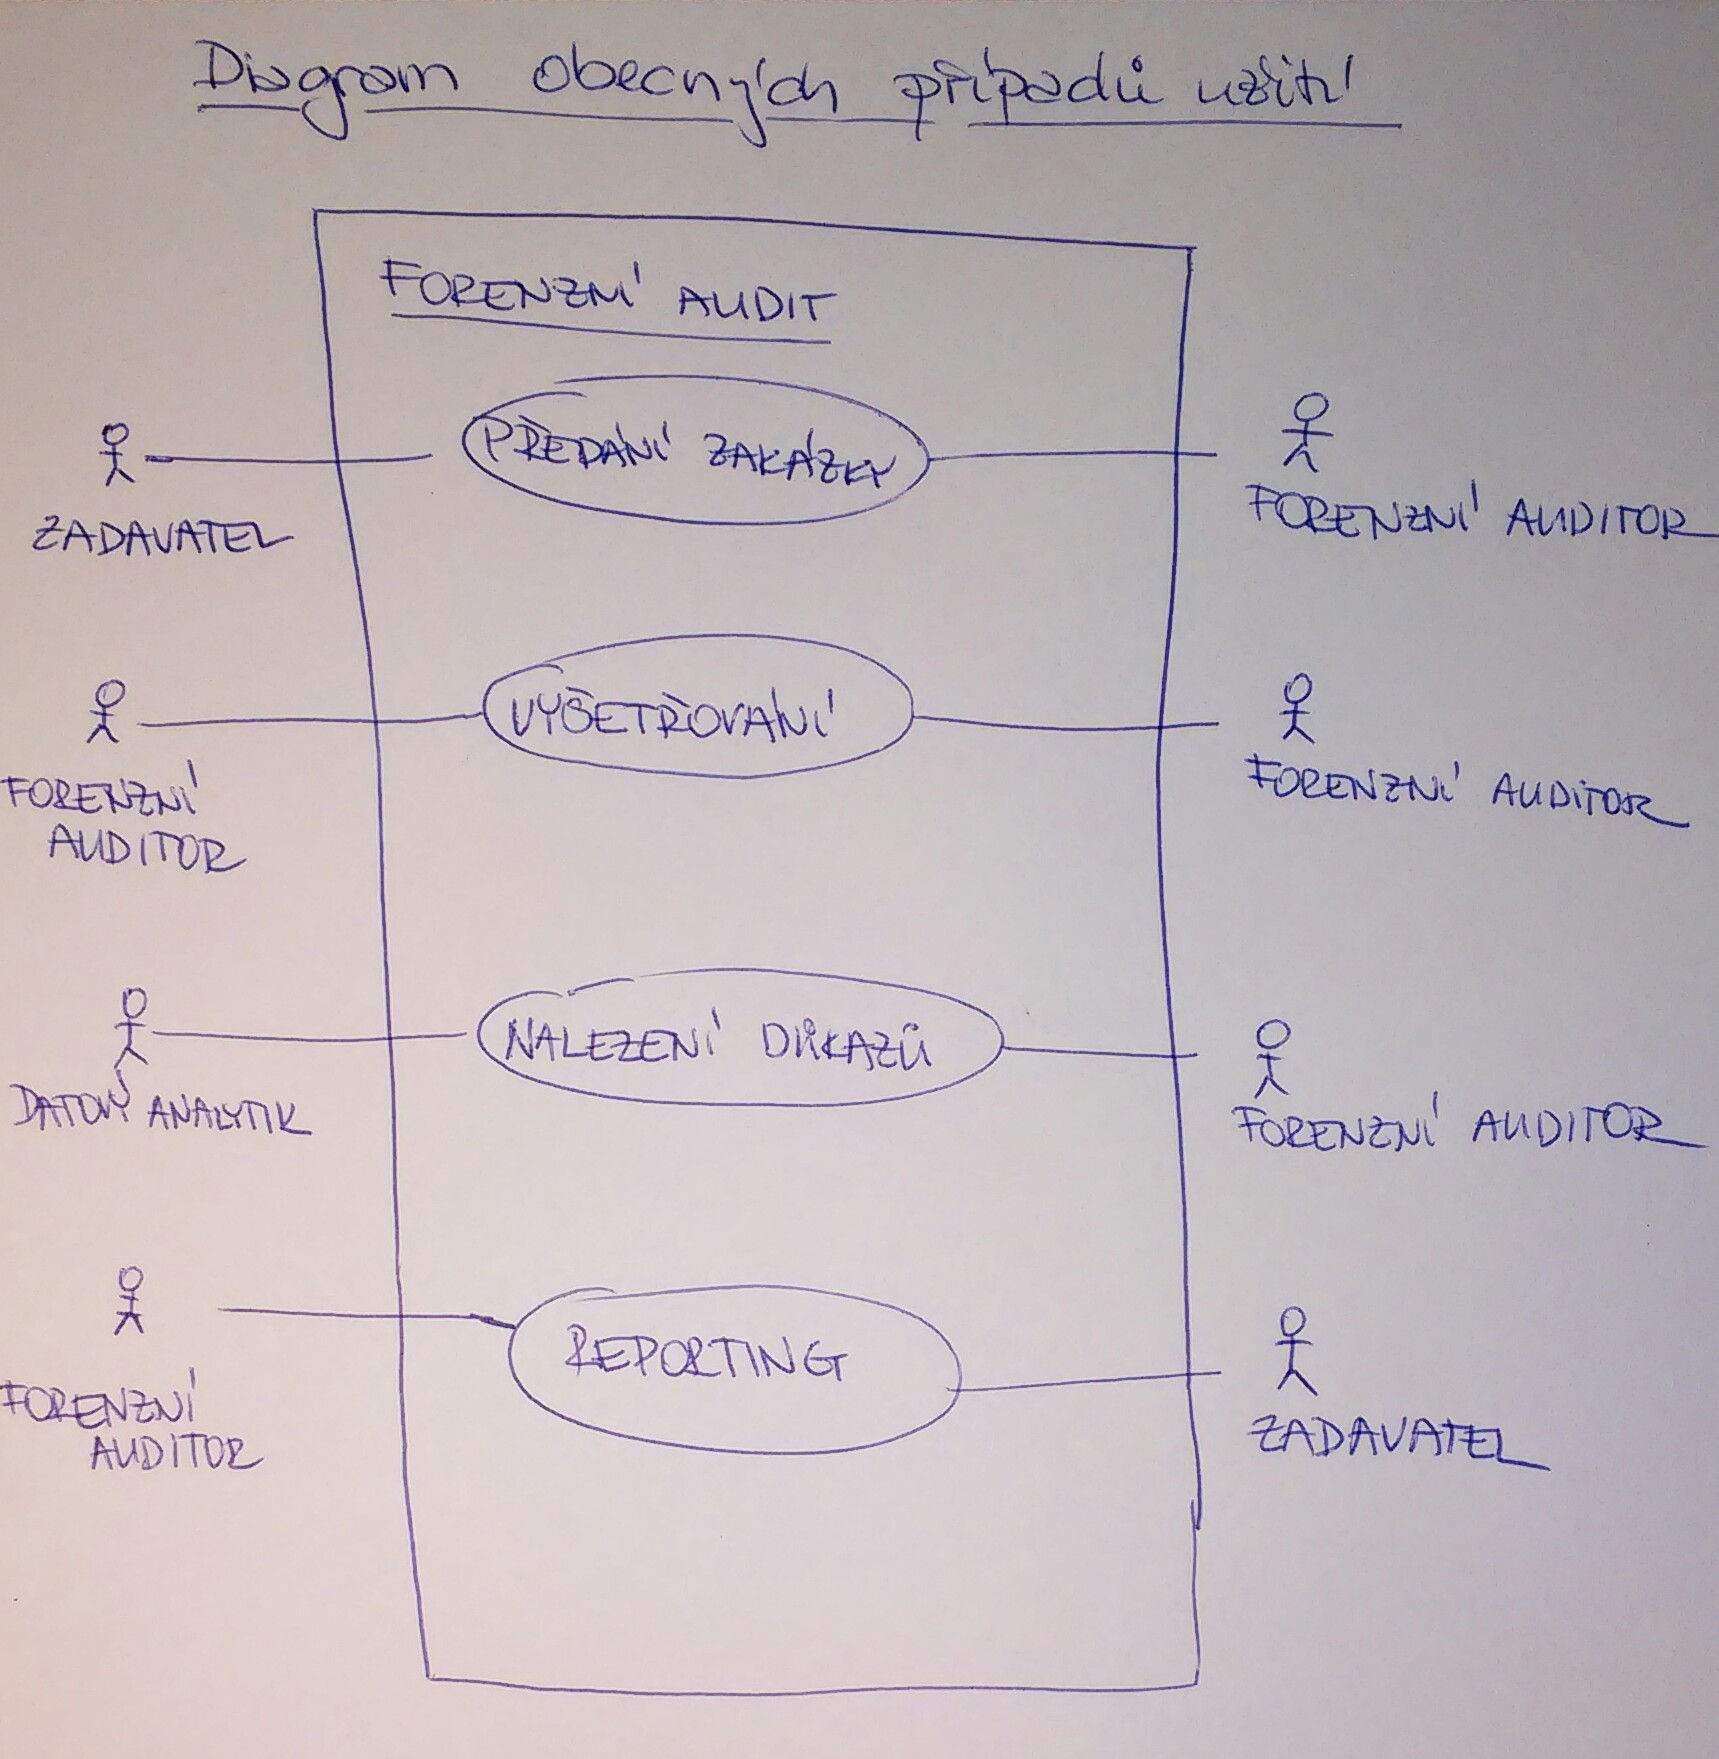
\includegraphics[width=1.0\textwidth]{img/fotky/20151007_000323.jpg}
	\end{center}
	\caption{\komentar{Velky obrazek vsech zainteresovanych stran - f.auditor, datovy analytik pro FA, zakaznik (zadavatel, materska spolecnost)}}
\end{figure}

